% Kiosk manual - Pump control box.
% Written by Christopher Thomas.

\chapter{Pump Control Box}
\label{sect-pumpbox}

\section{Overview}
\label{sect-pumpbox-over}

The pump control box allows the reward pump to be controlled by a 5V
active-high signal over BNC for automated rewards and by pressing a button 
on a fob for manual rewards. A schematic for the pump control box is
shown in Figure \ref{fig-pumpbox-schem}.

\textbf{NOTE} -- While a similar 1/4'' plug is used for old and new boxes,
cable plugs wired for old control boxes are \textbf{NOT} compatible with
the current control box, and vice versa. New cables use a stereo plug with
+15~V on the ring.

A diagram of box cutouts is shown in Figure \ref{fig-pumpbox-boxes}. A bill
of materials is given in Table \ref{tab-pumpbox-bom}.

\begin{figure}[h]
\begin{center}
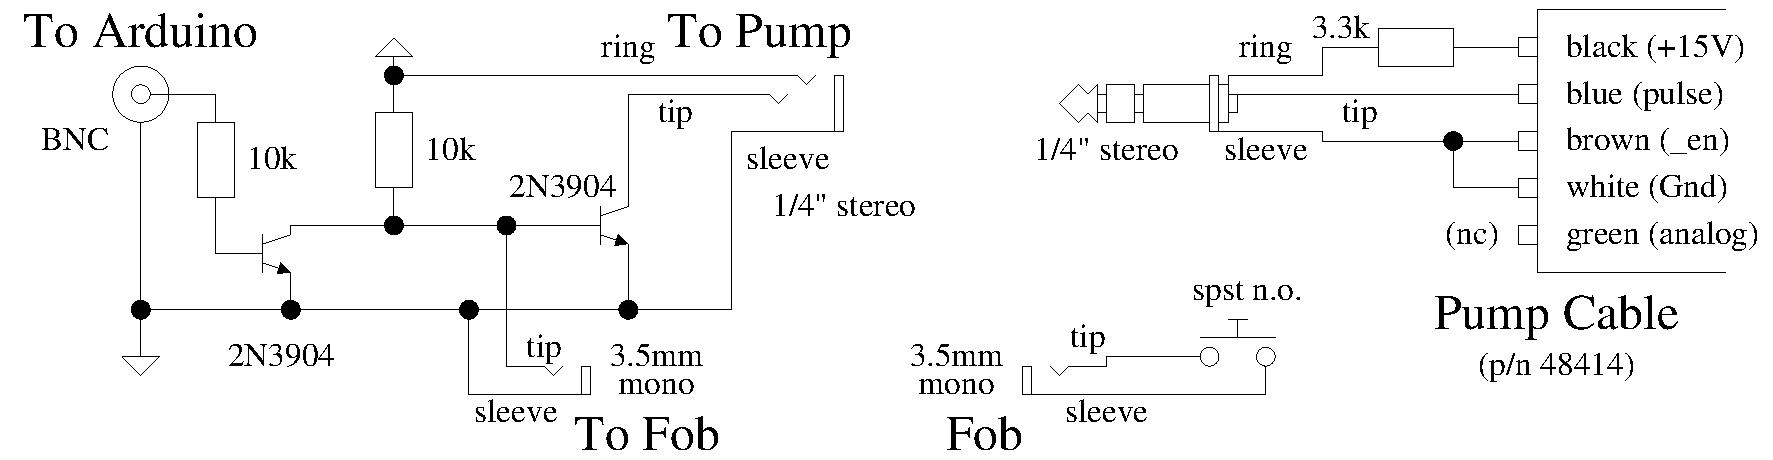
\includegraphics[width=0.95\columnwidth]
{figs-pump/pump-box-v1-schem.pdf}
\end{center}
\caption{Pump control box schematic.}
\label{fig-pumpbox-schem}
\end{figure}

\begin{figure}[h]
\begin{center}
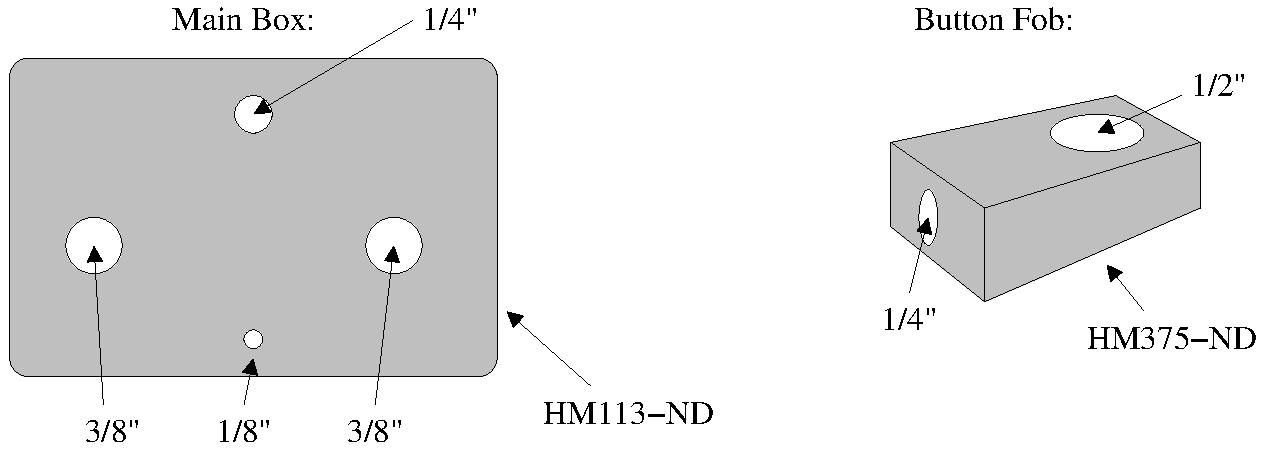
\includegraphics[width=0.8\columnwidth]
{figs-pump/pump-box-v1-mech-notitle.pdf}
\end{center}
\caption{Pump control box cutouts.}
\label{fig-pumpbox-boxes}
\end{figure}

\begin{table}[h]
\begin{center}
\begin{tabular}{llr}
\hline
\textbf{Item} & \textbf{Digikey p/n} & \textbf{Quantity} \\
\hline
box 3.25x2.25x1.5''		& HM113-ND	& 1	\\
box 2x1.5.0.75''		& HM375-ND	& 1	\\
transistor NPN TO-92		& 2N3904FS-ND	& 2	\\
resistor 1/4 W 10 kohm		& 10.0KXBK-ND	& 2	\\
resistor 1/4 W 3.3 kohm		& 3.3KXBK-ND	& 1	\\
proto board 1x1''		& 1568-1652-ND	& 1	\\
screw 4-40 nylon 1/4''		& H542-ND	& 1	\\
standoff nylon 4-40 F/F 1/2''	& 36-1902C-ND	& 1	\\
screw metal 4-40 3/8''		& HM1456-ND	& 1	\\
jack BNC panel mount		& ARFX1064-ND	& 1	\\
jack audio 1/4'' stereo panel	& SC1563-ND	& 1	\\
plug audio 1/4'' stereo		& SC1081-ND	& 1	\\
jack audio 3.5mm mono panel	& SC1455-ND	& 2	\\
cable audio 3.5mm M/M 10'	& TL634-ND	& 1	\\
button spst-no panel mount	& CW158-ND	& 1	\\
cable M12 rev key to wire	& $^\dagger$	& 1	\\
\hline
\multicolumn{3}{p{0.8\columnwidth}}
{$^\dagger$Sold by LMI as part number 48414; may be sourced more cheaply as
MEC-5FP-2M from www.mencom.com. These have a ``5 pole reverse-keyed'' M12
connector.} \\
\end{tabular}
\end{center}
\caption{Pump control box bill of materials.}
\label{tab-pumpbox-bom}
\end{table}

\clearpage
\section{Pump Cable Plug}
\label{sect-pumpbox-plug}

Assembly steps for the pump cable plug are shown below. Use of
$\frac{1}{8}$'' heat shrink tubing is strongly recommended to avoid shorts
within the plug housing.

\begin{itemize}
%
\item Trim wires to appropriate lengths, and feed cable through backshell.

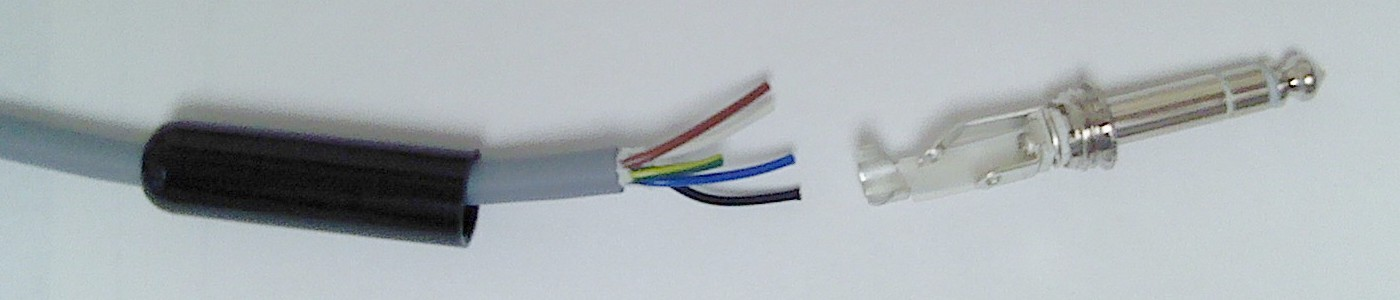
\includegraphics[width=0.8\columnwidth]
{photos/pump-box-20181030/plug-started.jpg}

\item Cap green wire with heat shrink, twist brown and white wires together
and tin, tin blue wire, solder resistor to black wire.

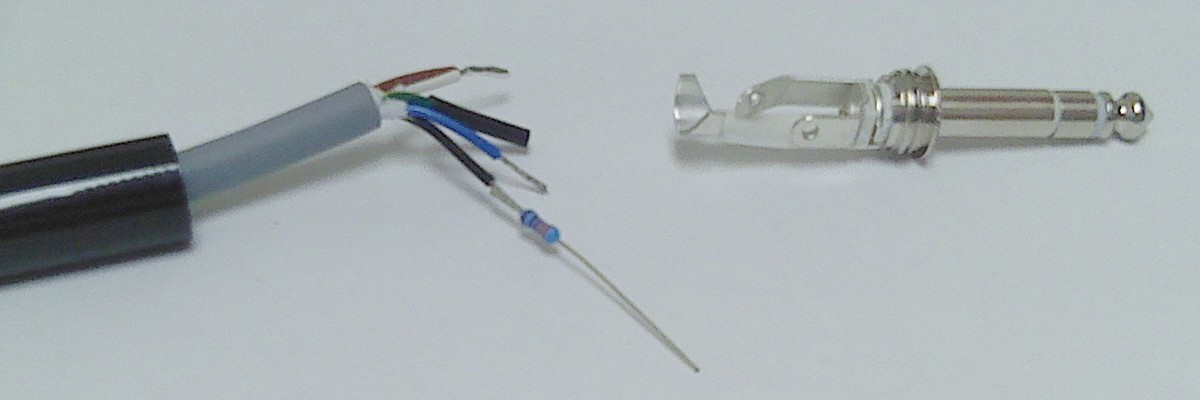
\includegraphics[width=0.8\columnwidth]
{photos/pump-box-20181030/plug-midway.jpg}

\item Cover resistor connection with heat shrink, solder blue wire,
resistor lead, and brown/white wire pair to appropriate lugs.

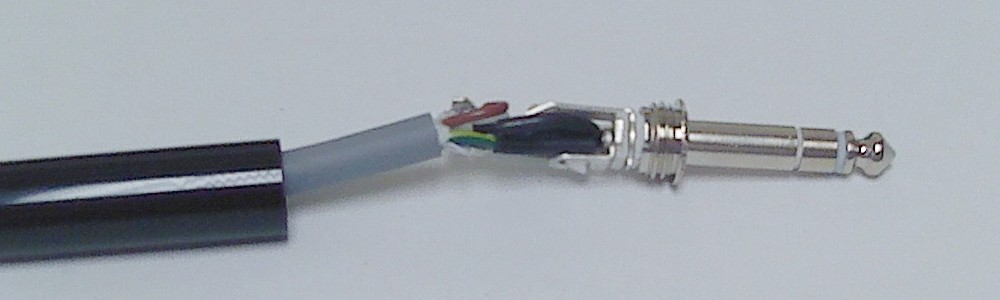
\includegraphics[width=0.8\columnwidth]
{photos/pump-box-20181030/plug-done.jpg}

\item Crimp collar around wires and screw backshell on to plug.

\textbf{NOTE} - ideally the wires would be short enough that the collar is
crimped to the jacket rather than to the wire bundle.
%
\end{itemize}

\clearpage
\section{Circuit Board}
\label{sect-pumpbox-board}

Assembly steps for the circuit board are shown below. The prototyping board
trace pattern and one possible layout are shown in Figure
\ref{fig-pumpbox-protoboard}.

\begin{figure}
\begin{center}
\begin{tabular}{ccc}
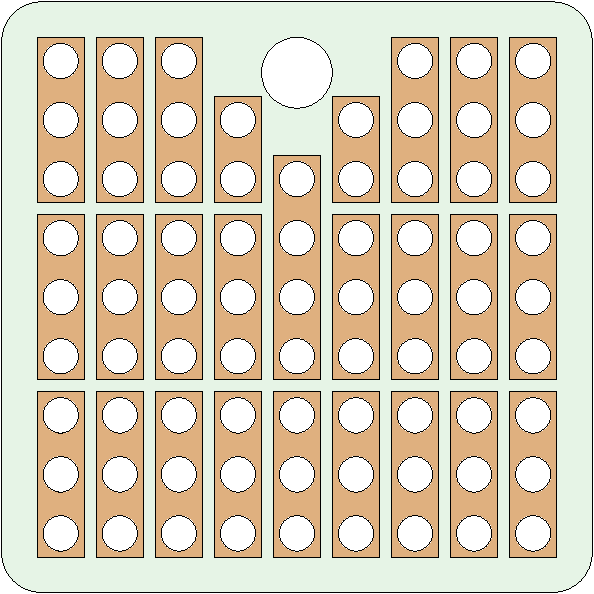
\includegraphics[height=2in]
{figs-pump/pump-box-v1-breadboard.pdf}
& ~ &
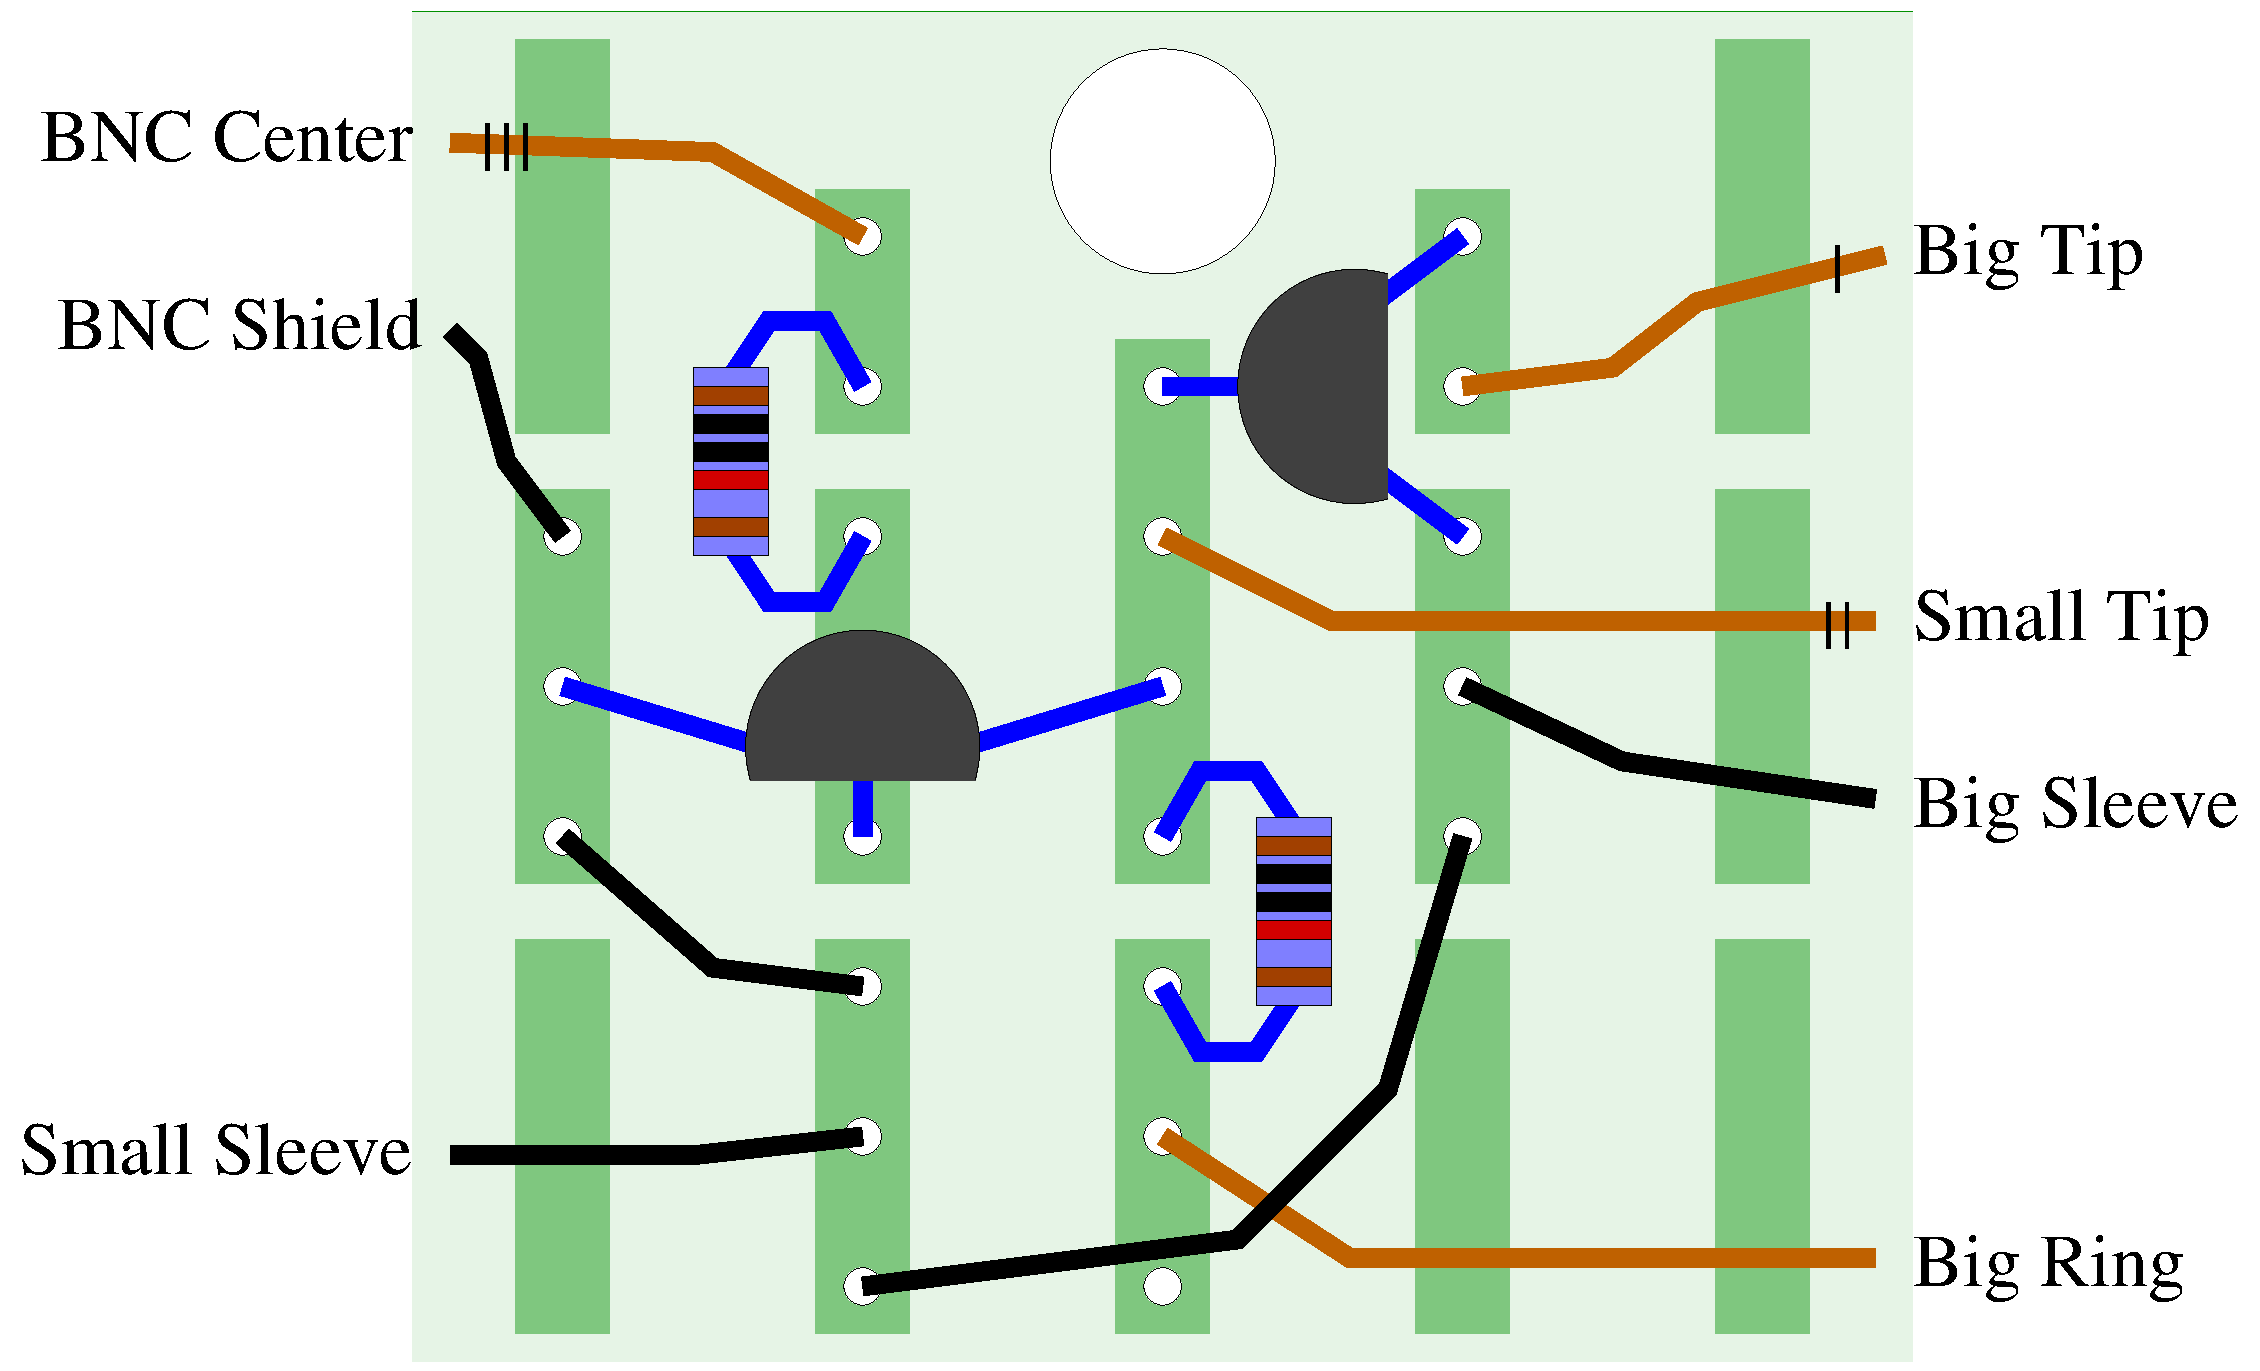
\includegraphics[height=2in]
{figs-pump/pump-box-v1-bblayout.pdf}
\\
\end{tabular}
\end{center}
\caption{Prototyping board and one possible pump control circuit layout.}
\label{fig-pumpbox-protoboard}
\end{figure}

\begin{itemize}
%
\item Solder transistors and resistors.

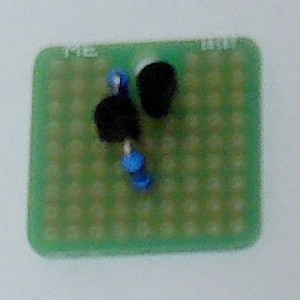
\includegraphics[height=2in]
{photos/pump-box-20181112/board-comps.jpg}

\item Solder signal and power wires. Marking is encouraged to keep track
of which are which.

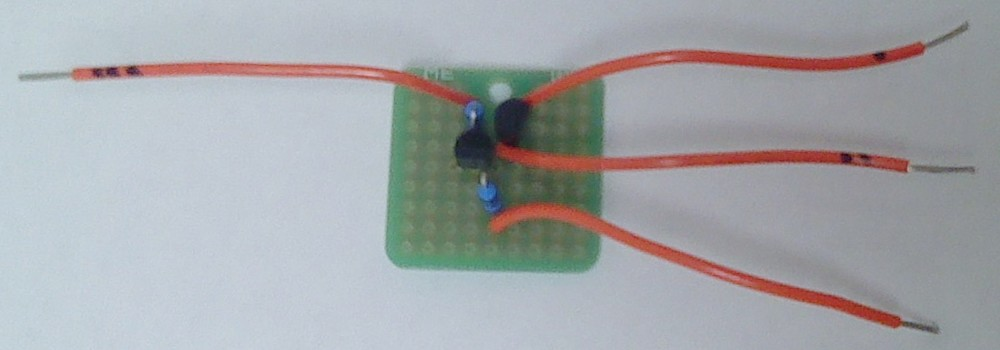
\includegraphics[height=2in]
{photos/pump-box-20181112/board-orange.jpg}

\clearpage
\item Solder ground wires.

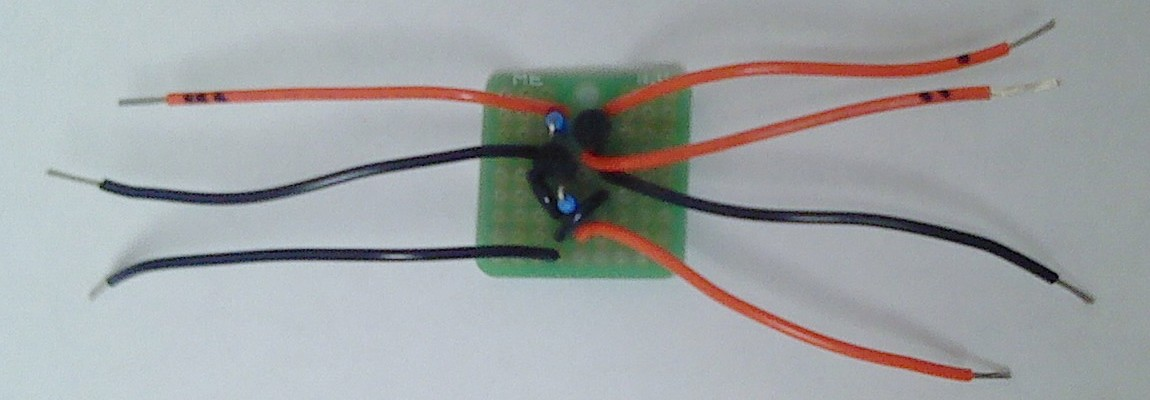
\includegraphics[height=2in]
{photos/pump-box-20181112/board-black.jpg}

\item Solder jacks to wires. Make sure to thread BNC hardware over the BNC
signal wire and to insert the BNC connector in the faceplate before soldering.

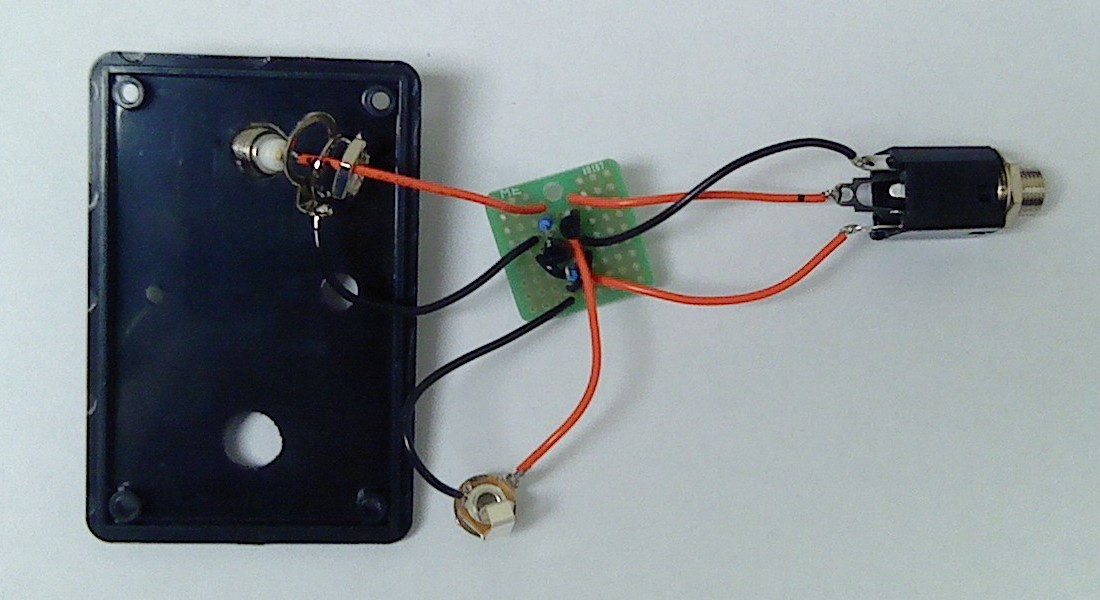
\includegraphics[height=3in]
{photos/pump-box-20181112/board-conns.jpg}

\item Screw circuit board to faceplate.

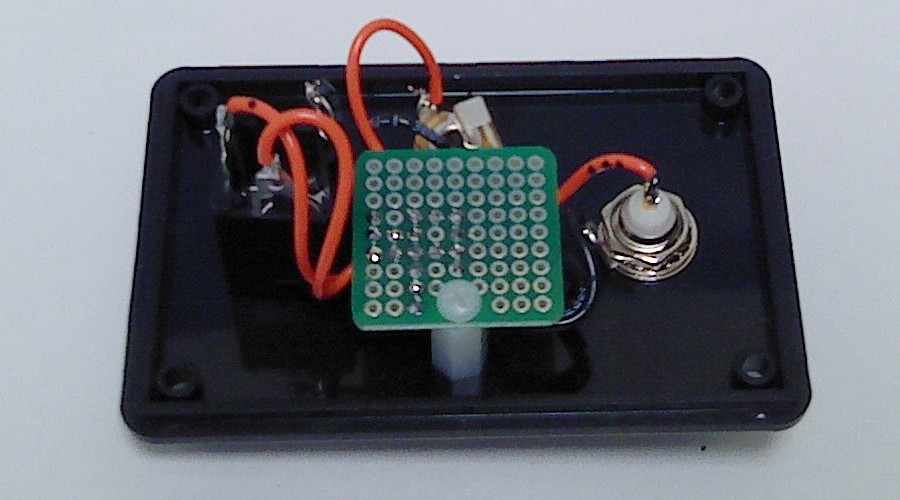
\includegraphics[height=2in]
{photos/pump-box-20181030/board-done.jpg}
%
\end{itemize}

%
% This is the end of the file.
